\documentclass[tikz,border=7pt]{standalone}

\usepackage{amsmath}
\usepackage{bm}
\usetikzlibrary{arrows.meta,calc}

% Blue used for the coordinate frames in the reference figure.
\definecolor{frameblue}{RGB}{48,52,255}
\definecolor{linkfill}{RGB}{249,249,249}

\tikzset{
  linkbody/.style={
    draw=black,
    fill=linkfill,
    line width=0.85pt,
    rounded corners=3.2mm
  },
  frameaxis/.style={
    draw=frameblue,
    line width=1.15pt,
    line cap=round,
    -{Stealth[length=2.4mm,width=1.9mm]}
  },
  positionline/.style={
    draw=black,
    line width=0.55pt
  }
}

\begin{document}
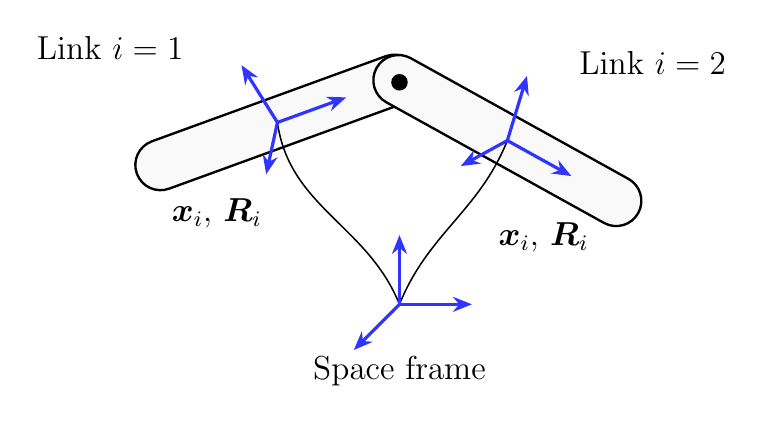
\begin{tikzpicture}[x=1cm,y=1cm]

  % Geometric centers of the links, joint, and global-frame origin.
  \coordinate (C1) at (-1.55, 0.66);
  \coordinate (C2) at ( 1.37, 0.43);
  \coordinate (J)  at (-0.00, 1.17);
  \coordinate (G)  at ( 0.00,-1.65);

  % Draw link i=1 first.
  \begin{scope}[shift={(C1)},rotate=20]
    \path[linkbody] (-1.90,-0.32) rectangle (1.90,0.32);
  \end{scope}

  % Link i=2 is shifted slightly upward and to the left. It is drawn above
  % link i=1, with the joint centered between its upper and lower borders.
  \begin{scope}[shift={(C2)},rotate=-29]
    \path[linkbody] (-1.90,-0.32) rectangle (1.90,0.32);
  \end{scope}

  % Position curves are drawn above both bodies and remain visible up to the
  % origins of the corresponding body-fixed frames.
  \draw[positionline] (G) to[out=112,in=-82] (C1);
  \draw[positionline] (G) to[out= 68,in=-112] (C2);

  % Three-dimensional body-fixed frame at the exact center of link i=1.
  \begin{scope}[shift={(C1)},rotate=20]
    \draw[frameaxis] (0,0) -- ( 0.93, 0.00);
    \draw[frameaxis] (0,0) -- (-0.18, 0.84);
    \draw[frameaxis] (0,0) -- (-0.36,-0.57);
  \end{scope}

  % Three-dimensional body-fixed frame at the exact center of link i=2.
  \begin{scope}[shift={(C2)},rotate=-29]
    \draw[frameaxis] (0,0) -- ( 0.93, 0.00);
    \draw[frameaxis] (0,0) -- (-0.18, 0.84);
    \draw[frameaxis] (0,0) -- (-0.36,-0.57);
  \end{scope}

  % Revolute joint, drawn above both links.
  \fill[black] (J) circle[radius=0.105];

  % Body and state labels requested for the thesis notation.
  \node[font=\large,anchor=east] at (-2.62,1.60) {Link $i=1$};
  \node[font=\large,anchor=west] at ( 2.16,1.42) {Link $i=2$};
  \node[font=\large] at (-2.32,-0.50) {$\bm{x}_{i},\,\bm{R}_{i}$};
  \node[font=\large] at ( 1.83,-0.80) {$\bm{x}_{i},\,\bm{R}_{i}$};

  % Three-dimensional global coordinate frame in projected form.
  \draw[frameaxis] (G) -- ++(0.92,0.00);
  \draw[frameaxis] (G) -- ++(0.00,0.88);
  \draw[frameaxis] (G) -- ++(-0.58,-0.58);
  \node[font=\large,anchor=north] at ($(G)+(0,-0.54)$) {Space frame};

\end{tikzpicture}
\end{document}
